\documentclass[paper=letter, fontsize=12pt]{article}

\usepackage{amsmath,amsfonts,amsthm, amssymb} % Math packages
\usepackage{stmaryrd}
\usepackage[shortlabels]{enumitem}
\usepackage[pdftex]{graphicx}
\usepackage{booktabs}
\usepackage{placeins}
\usepackage{algpseudocode}
\usepackage[margin=1in]{geometry}
\usepackage{listings}
\usepackage{mdframed}
\usepackage{tcolorbox}
\usepackage{float}
\usepackage{subcaption}
\usepackage{url}
\usepackage{hyperref}

\usepackage{mathtools}
\DeclarePairedDelimiterX{\norm}[1]{\lVert}{\rVert}{#1}
\DeclarePairedDelimiterX{\abs}[1]{\lvert}{\rvert}{#1}
\DeclareMathOperator*{\argmin}{arg\,min}
\DeclareMathOperator{\spn}{span}
\DeclareMathOperator{\rct}{rect}
\DeclareMathOperator{\support}{support}
\DeclareSymbolFont{matha}{OML}{txmi}{m}{it}% txfonts
\DeclareMathSymbol{\varv}{\mathord}{matha}{118}
\DeclareMathOperator{\E}{\mathbb{E}}
\DeclareMathOperator{\Tr}{Tr}

\newcommand{\ceil}[1]{\lceil #1 \rceil}
\newcommand{\floor}[1]{\lfloor #1 \rfloor}
\newcommand{\Lapl}{\mathcal{L}}
\newcommand{\reals}{\mathbb{R}}
\newcommand{\complexes}{\mathbb{C}}
\newcommand{\ints}{\mathbb{Z}}
\newcommand{\innerp}[2]{\langle #1, #2 \rangle}
\newcommand{\vecii}[2]{\begin{bmatrix} #1 \\ #2 \end{bmatrix}}
\newcommand{\veciii}[3]{\begin{bmatrix} #1 \\ #2 \\ #3 \end{bmatrix}}
\newcommand{\rect}[1]{\rct \left( #1 \right)}
\newcommand{\pw}[1]{\begin{cases} #1 \end{cases}}
\newcommand{\Mod}[1]{\ \text{mod}\ #1}
\newcommand{\sumN}{\sum\limits_{n=0}^{N-1}}
\newcommand{\sumK}{\sum\limits_{k=0}^{N-1}}
\newcommand\given[1][]{\:#1\vert\:}

\graphicspath{{img/}}

\title{CS 543 - Progress Report}
\author{
        Dario Aranguiz \\
        Cu-Khoi-Nguyen Mac
        }
\date{\today}


%%% Begin document
\begin{document}
\maketitle
% \pagebreak

\section{Updated statement of the project definition and goals}

\textit{We have no particular changes to our project scope. Our project
proposal is copied below for posterity.}

For our final project, we plan on implementing and exploring extensions of the
2015 paper \textit{Multimodal Deep Learning for Robust RGB-D Object
Recognition} \cite{Eitel2015} by Eitel et al. Our research group has recently
taken interest in the capabilities of depth cameras, and as such we have
various time of flight and structured-light depth sensors. Our group members
have done quite a bit of work in facial recognition and related areas using
depth, but an area we have yet to explore is augmenting traditional RGB-based
object recognition approaches with depth information. To this end, we have
chosen a recent paper from IROS 2015 that approaches the age-old problem of
object recognition with two new modalities, depth and deep learning.

The motivation for this technique is as follows. Convolutional Neural Networks
(CNNs) have proven remarkably useful for object recognition in the last few
years, with large companies such as Microsoft and Google pouring resources
into training more efficient networks. We are also interested in this problem,
but unlike Microsoft and Google, we do not have a GPU farm at our disposal to
train networks ad-infinitum. This prompts an interesting question; how can we
utilize pre-trained ImageNet networks while incorporating depth information?
CNNs require a fixed-size input, and most pre-trained networks have only been
trained on three-channel information. That constraint is the primary
motivation behind Eitel et al's technique.

To get around this problem, two separate three-channel networks are used: one
to process the incoming RGB images, and another to process the incoming depth
information. This depth information is transformed from single-channel
distance information to a three-channel RGB image using a depth-to-color
heatmap, the intuition being that useful features such as edges and corners
are preserved in this transformation. The final fully-connected layers of each
of these networks are then removed, and the second-to-last activation layers
are fed into a single large classification layer, merging the two networks.
Additional preprocessing is also done, but the system functions loosely as
described.

Our expected final outcome is to have a fully-functioning system that can
distinguish between objects from the Washington RGB-D Object Dataset. At
minimum, we aim to replicate the paper and get a recognition system of our own
running locally. We have a few stretch goals, listed in order of expected
difficulty:

\begin{enumerate}

    \item \textbf{Different Backends} - The current most-frequently used
    network backend is a package called Theano. However, Google recently
    released their own open-source Machine Learning backend called
    TensorFlow. It would be interesting to compare the efficacy of these two
    systems with our project.

    \item \textbf{Different Classification Layers} - In the paper, the authors
    recommend using a single fully-connected layer at the end of the pipeline
    for classification. It would be interesting to see how this scheme
    compares with other classification methods such as logistic regression,
    SVM, Random Forests, and others.

    \item \textbf{Different Preprocessing Schemes} - The authors prescribe a
    number of preprocessing techniques to convert depth images from one-channel
    data to three-channel data, but other preprocessing techniques have been
    used in the past to do this as well.

    \item \textbf{Network Modifications} - This is by and large our most
    ambitious stretch goal. The two-network system is core to the authors'
    architecture, but we would be interesting in exploring different ways of
    fusing depth data with traditional RGB data. This comes with a number of
    challenges, the least being that any modification to a pretrained ImageNet
    network would eliminate the benefit of using a pretrained network at all.

\end{enumerate}


\section{Current member roles and collaboration strategies}

As mentioned in the proposal, this project is not easily split into modules.
Dario has been helping with the actual Keras implementation of the stream
network, and Mac has been completing the preprocessing stages as well as the
actual Keras implementation. Code is shared in a GitHub repository, whereas
copies of the dataset are only stored locally. As for communication, we maintain
an open communication channel using Slack as well as simply sitting near each
other in our group's office. To that end, we do not have regular meetings, but
rather ad-hoc meetings whenever one of us gets stuck.


\section{Proposed approach}

Proposed approach in the form of a detailed outline, pseudocode, or prose description. Be specific about how you plan to implement each step with references, pointers to external code, etc. One or more references are required at this stage.

TODO



\section{Data}

Following the proposed approach by Eitel et al. \cite{Eitel2015}, we decide to
use Washington's RGB-D object dataset \cite{Lai2011} for training and testing.
The dataset contains 300 household objects (instances) divided into 51
categories. Each instance has three different takes, each records a full turn-
around rotation of the object. A sample of the full database includes images of
color, depth, mask (as seen in Figure \ref{fig:banana}), and a text file
recording the top-left corner of the object.

\begin{figure}[htbp]
	\centering
	\begin{subfigure}[b]{0.32\linewidth}
		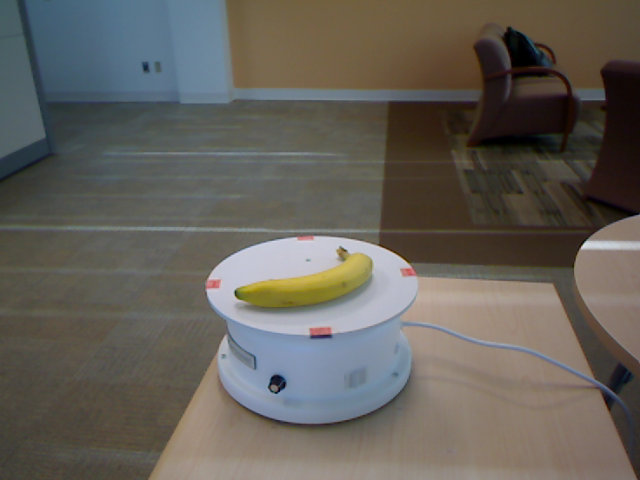
\includegraphics[width=\textwidth]{banana_1_1_1}
		\caption{Color image}
	\end{subfigure}
	\begin{subfigure}[b]{0.32\linewidth}
		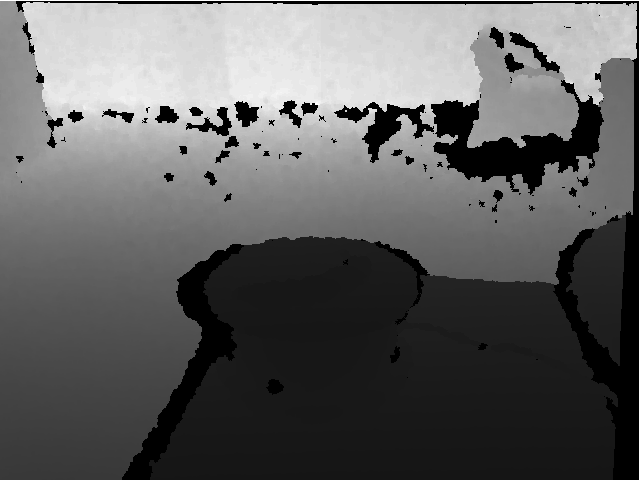
\includegraphics[width=\textwidth]{banana_1_1_1_depth}
		\caption{Depth image}
	\end{subfigure}
	\begin{subfigure}[b]{0.32\linewidth}
		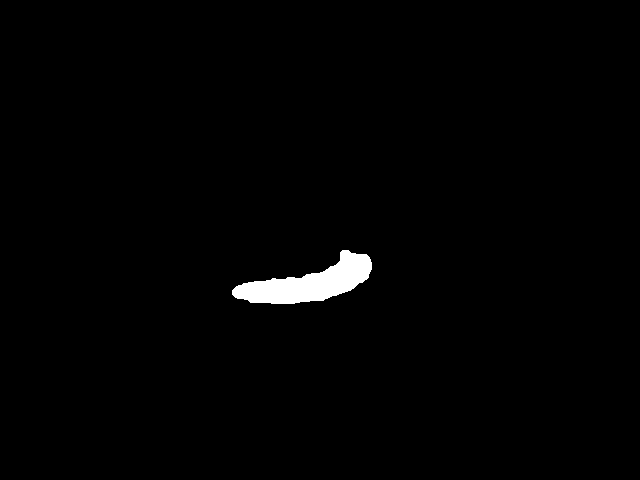
\includegraphics[width=\textwidth]{banana_1_1_1_mask}
		\caption{Mask}
	\end{subfigure}

	\caption{A banana sample of Washington's RGB-D object dataset. The depth image is rescaled to the range [0, 255] to visual the information.}
	\label{fig:banana}
\end{figure}

To speed up the process of testing our system's runnability, we pick out 15 instances from 5 different categories (3 each), namely \texttt{apple}, \texttt{ball}, \texttt{banana}, \texttt{bell\_pepper}, and \texttt{binder}. After the system is fully functional, we will expand the training list to the whole dataset.


\section{Initial results}
\subsection{Data preprocessing}
We use the provided masks and top-left corners to remove unnecessary information from color and depth images (Figure \ref{fig:banana_crop}). Top bottom-right corner if dynamically found, depending on each sample. According to Eitel et al. \cite{Eitel2015}, they convert the depth images into color ones using colorjet mapping as they want to have the same training mechanism for both color and depth. We inherit this idea and apply the same depth colorizing technique. The images are then rescaled to 227x227 (Figure \ref{fig:banana_resize}) by replicating the longer side from the cropped images. This help to maintain the object in the center without deformation after rescaling.

\begin{figure}[htbp]
	\centering
	\begin{subfigure}[b]{0.32\linewidth}
		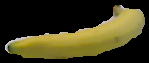
\includegraphics[width=\textwidth]{banana_1_1_1_crop}
		\caption{Color image}
	\end{subfigure}
	\begin{subfigure}[b]{0.32\linewidth}
		
\includegraphics[width=\textwidth]{banana_1_1_1_depth_crop}
		\caption{Depth image}
	\end{subfigure}
	\caption{Cropping banana sample after applying mask.}
	\label{fig:banana_crop}
\end{figure}

\begin{figure}[htbp]
	\centering
	\begin{subfigure}[b]{0.32\linewidth}
		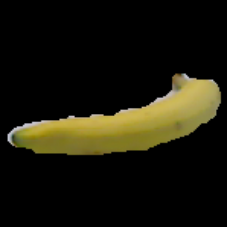
\includegraphics[width=\textwidth]{banana_1_1_1_resize}
		\caption{Color image}
	\end{subfigure}
	\begin{subfigure}[b]{0.32\linewidth}
		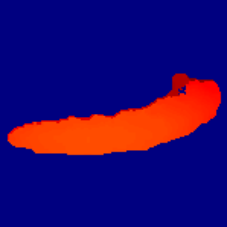
\includegraphics[width=\textwidth]{banana_1_1_1_depth_resize}
		\caption{Depth image (after colorizing)}
	\end{subfigure}
	\caption{Rescaling banana sample to 227x227 by replicating the longer side.}
	\label{fig:banana_resize}
\end{figure}

\subsection{Model architecture}
Figure \ref{fig:architecture_eitel} illustrates the network architecture proposed by Eitel et al. \cite{Eitel2015}. There are two separate stream models, corresponding to color and depth channels. Each stream contains 5 convolution (from \texttt{conv-1} to \texttt{conv-5}) and 2 fully connected layers (\texttt{fc6} and \texttt{fc7}). The streams are fused together by one fusion layer (\texttt{fc-fus}) and classified by \texttt{class} layer.
\begin{figure}[htbp]
	\centering
	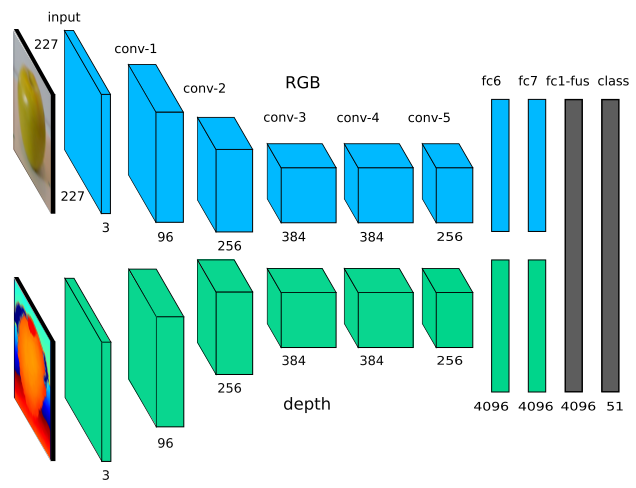
\includegraphics[width=.7\textwidth]{architecture}
	\caption{Model architecture proposed by Eitel et al. \cite{Eitel2015}.}
	\label{fig:architecture_eitel}
\end{figure}

Figure \ref{fig:fusion_model} shows our model, constructed by following the description in Figure \ref{fig:architecture_eitel}. The model is plotted using visualizer package of Keras. Using Keras, each stream is constructed using \texttt{Sequential()} model and the fusion layer is created by \texttt{Merge()} layer. We propose to augment each convolutional layer (\texttt{Convolution2D()}) with a maxpooling (\texttt{MaxPolling2D()}) and a dense sampling layer (\texttt{Dense()}) to reduce the risk of over-fitting and decrease memory usage.

In fact, there are two different training process: one to find the weights of stream model and one for the fusion model. To train a stream model, we create an architecture similar to a branch in Figure \ref{fig:fusion_model} and add one classifier at the end (Figure \ref{fig:stream_model}). The weights of trained streams are reused to initialize the two branches of the whole network.

\begin{figure}[htbp]
\centering
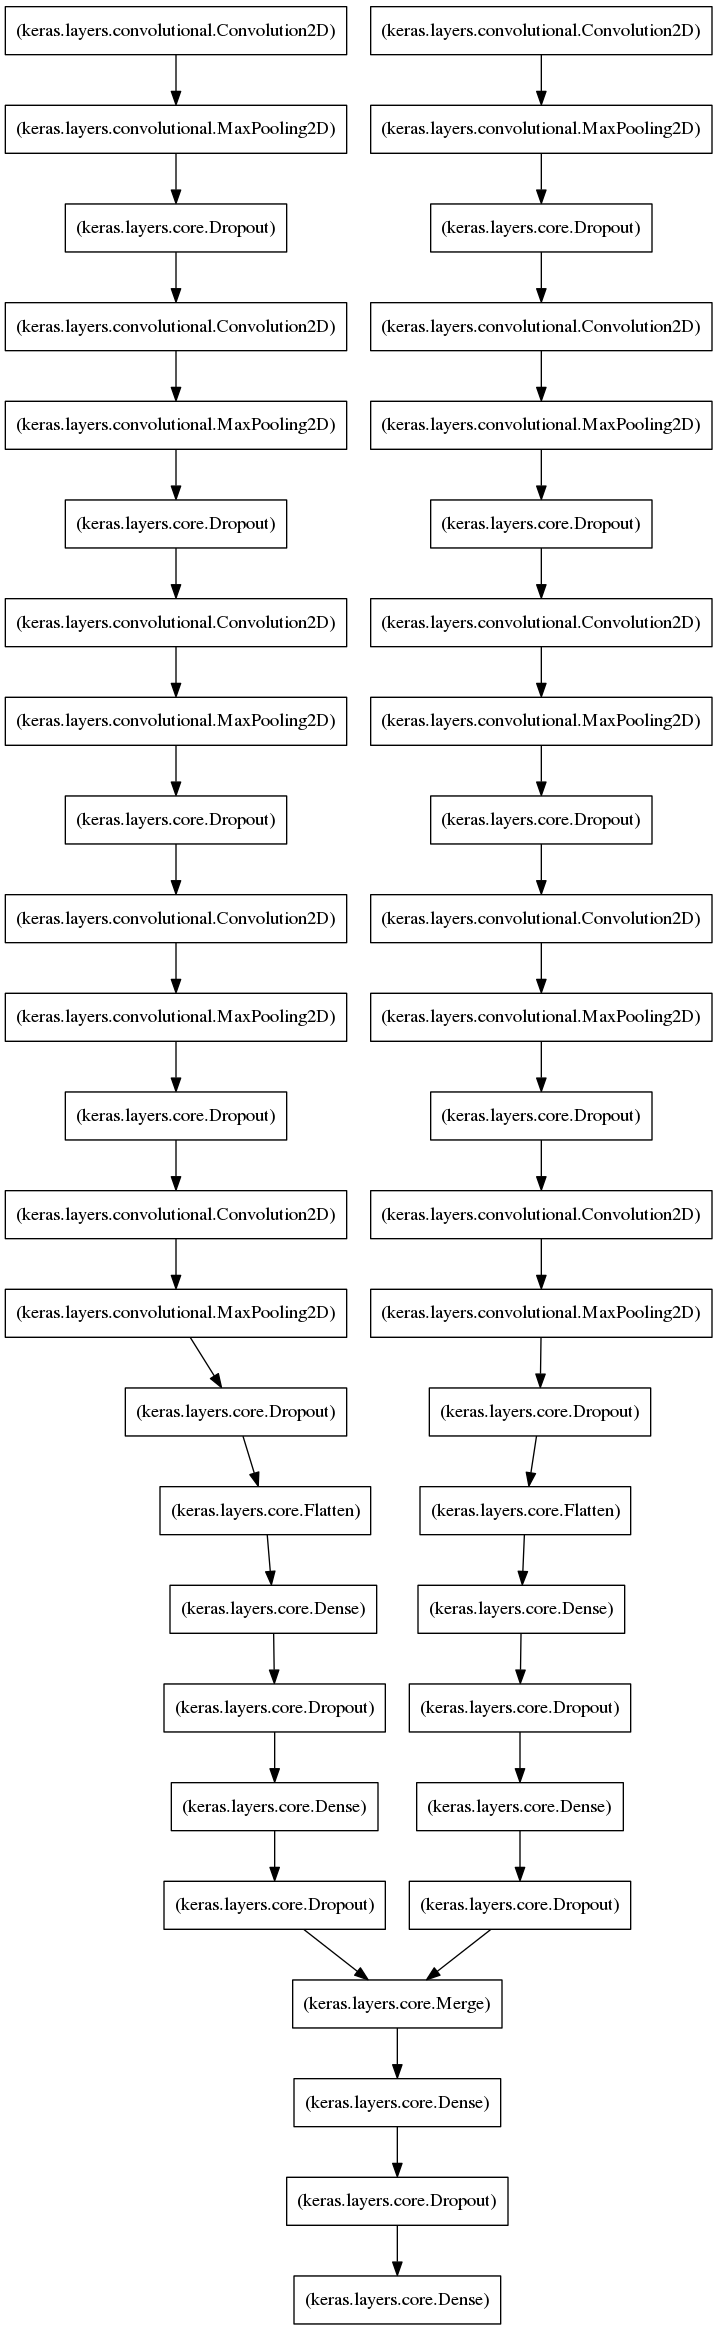
\includegraphics[width=.42\textwidth]{fusion_model}
\caption{Fusion model with RGB and depth streams.}
\label{fig:fusion_model}
\end{figure}

\begin{figure}[htbp]
	\centering
	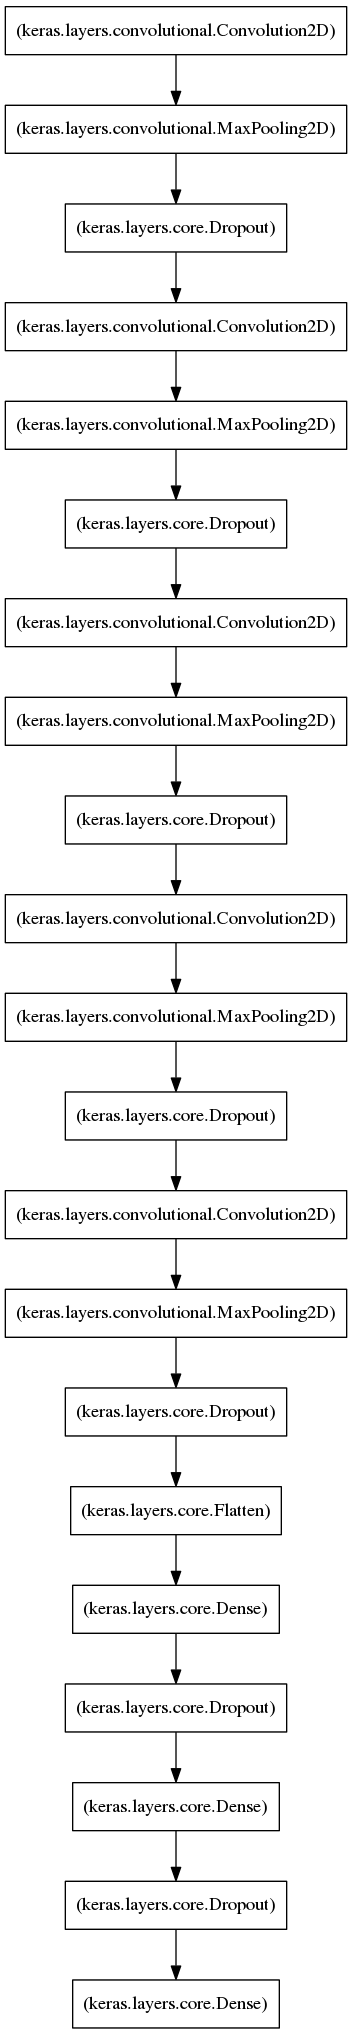
\includegraphics[width=.24\textwidth]{stream_model}
	\caption{Single stream model.}
	\label{fig:stream_model}
\end{figure}

\subsection{Other accomplishments}
Beside data preprocessing and model construction, we have also successfully configured a GPU environment for Keras/Theano to speed up training process. In addition, the paper mentions about using CaffeNet to initialize the network. However, this pretrained network has to be converted to Keras format before loading. We utilize a modified version of Keras that includes conversion package, provided by Bolanos \cite{Bolanos2016}.

\section{Current reservations and questions}
(if any)

\bibliographystyle{ieeetr}
\bibliography{mybib}


%%% End document
\end{document}